%%%%%%%%%%%%%%%%%%%%%%%%%%%%%%%%%%%%%%%%%%%%%%%%%%%%%%%%%%%%

\chapter{Background and Related Work}\label{chap:background}
To obtain entity embeddings we use GloVe and word2vec on annotated corpus. We furthur extract an implicit network of named entities, namely LOAD, and embed the graph to generate the embeddings. The facetted models also extend the GloVe and word2vec and apply graph-based embeddings. To provide a general background for all the methods used in this work the related work is organized as follows: first, a brief overview of the text preprocessing steps for NLP tasks is given, in which methods used extract information from text and generate the an implicit network is explained. In Section~\ref{sec:nn}  neural network based approaches for learning embeddings is explained. Since word2vec and GloVe are the building blocks of other models they are described in Section~\ref{sec:textual}. In this section, we also explain how edge weights of the implicit network can be used to generate a weighted adjacency matrix, which is comparable to a co-occurrence matrix in the GloVe model.  Finally, an overview of the graph embedding methods is given in Section~\ref{sec:graph}.
\section{Basics of Natural Language Processing}
The goal of NLP systems is to understand and derive meaning from human language. Textual data is a valuable source of information in NLP. Most of the World Wide Web is made of text, with websites like Twitter generating vast amounts every day. Analysing this content is, however, not a simple task. For example, text might contain ambiguity, in the sentence \emph{``I put my \textbf{wallet} in the  \textbf{car}.  \textbf{It} is green.''} In this sentence is not obvious if \emph{``it''} refers to the \emph{``car''} or the  \emph{``wallet''}. Moreover, humans often use homonyms (words having the same spelling but different meanings), metaphors and sarcasm, which makes text analysis a challenging task. 
\noindent
As machine learning systems rely on features, the most important step is to derive features from the text. There have been many models proposed for feature extraction, while none of them achieve the goal of fully characterizing a text, some are more useful than others. However, all features require the cleaning and preprocessing of the text. 

\subsection{Text cleaning }
Before any operation can be performed on text, each sentence has to be broken down to its atomic pieces. \emph{Tokenization} is the act of chopping sentence up into pieces, called \emph{tokens}.  For example, the sentence: \emph{Tokenization is widely used in Natural Language Processing}, can be tokenized as follows : 

\mybox{Tokenization} \mybox{is} \mybox{widely} \mybox{used} \mybox{in} \mybox{natural language processing}.\\
\\
As demonstrated in the example, splitting only on white spaces can also split what should be regarded as a single token. In a later section, we discuss \emph{named entity recognition} that eliminates such problems.  \\
\noindent
Text data has many inconsistencies that can cause algorithms trouble. Some common initial preprocessing steps are to convert all of the letters to lowercase and to remove punctuation. 
This makes sure that \emph{``analytics"}, \emph{``AnALYticS"}, \emph{``Analytics!"}, and \emph{``\#analytics"} are all considered the same word. Removing punctuation should be applied with care as in some cases, such as in case of Twitter \emph{``\#analytics"} is a message about analytics and should not be confused with \emph{``@analytics"}, which is a message to the  analytics account. For these reasons, the removal of punctuation should be tailored to the specific problem.\\
Additonally, words such as \emph{``are"} and \emph{``to"} are frequent in all documents but are only meaningful in a sentence. These are called \emph{stop-words} . Despite the high frequency, these words are unlikely to result into a meaningful feature for a machine learning system and are often removed. Same as the punctuation, removing stop words blindly may result in loss of valuable information. For example, \emph{``The Who"} is the name of a band, which by removing the stop-words, we remove both of these words, but it might have a significant meaning~\brackettext{\cite{edx}}. Hence, removing all stop-words is not always helpful, but it is generally a useful step. 

\subsection{Stemming and  lemmatization}
Another important preprocessing step is \emph{stemming} or \emph{lemmatization}. This step is motivated by the desire to represent words with different endings as the same word. There is no need for a distinction between \emph{argue}, \emph{argued}, \emph{argues}, and \emph{arguing}. They could all be represented by a common stem: \emph{argu}. This is called Stemming as it chops off the ends of words and often includes the removal of derivational affixes. Another approach is the use of Lemmatization, which uses the vocabulary and morphological analysis of words, normally aiming to remove inflectional endings only and to return the base or dictionary form of a word, which is known as the lemma. Lemmatization is a more complex task as it is necessary to have detailed dictionaries which the algorithm can look through to link the form back to its lemma. For instance:
Lemmatization of drank is drink~\brackettext{\cite{larson2010introduction}}. Although the LOAD network originally uses Stemming as a preprocessing step, to generate facetted embeddings, we use the complete word. Otherwise testing for the similarity of words, such as \emph{``larger"} and \emph{``large"} could not be achieved. 
\subsection{Part-Of-Speech tagging (POS-tagging)}
\emph{POS tagging} is the process of marking up a word in a text corresponding to a particular part of speech. Parts of speech are also known as \emph{word classes} or \emph{lexical categories} (e.g., noun, verb, adjective,~\dots). POS tags are useful because of a large amount of information they give about a word and its neighbors and also about the syntactic structure around the word. Parts of speech are useful features for finding named entities like people or organizations in text~\brackettext{\cite{DanielJurafsky2016}}. \emph{POS taggers} are the software used to assign tags to tokens using a finite predefined tagset. For English, the most commonly used tagset is the \textbf{Penn Treebank POS tagset} \footcite{https://www.ling.upenn.edu/courses/Fall_2003/ling001/penn_treebank_pos.html}. 
\subsection{Named entity recognition and  entity linkage}
\emph{Named entity recognition} (NER) or \emph{entity extraction} is an information extraction method that locates and classifies the named entities in text. Entities are classified into a set of pre-defined classes, such as the names of persons, organizations, locations, quantities and monetary values. In some case, temporal expressions are classified separately as well. Generally, anything that is not an entity per se is considered to be a term. Recognition of entities is difficult, partly because of ambiguity and mostly because of multiple surface forms. It is not always clear what is or is not an entity or what type it has. For example, the entity \emph{``Washington"} can be a name of a city, a person or even an organisation. NER identifies the occurrence or mention of a named entity in the text, but it does not identify which specific entity it is. \emph{Named entity linking} (NEL) or \emph{named entity disambiguation} (NED) is the task of mapping the found entities to a repository of entities. For this purpose, \emph{knowledge bases} are used, which contain rich information about the entities and their mutual relationships. NEL maps the found entities to their corresponding pair in the knowledge base~\brackettext{\cite{DBLP:journals/tkde/ShenWH15}}. To generate the LOAD network, both of these methods were used to identify and disambiguate entities in the given corpus. These entities form the networks nodes in later steps. 

\section{Neural Networks  in Natural Language Processing }\label{sec:nn}
Before the advancements in deep learning and neural networks, most NLP techniques were based on machine-learning approaches with linear models such as support vector machines or logistic regression, trained on very high dimensional and sparse feature vectors. Recently, the field has changed to use non-linear neural-network models over dense inputs. The most important advantage of such methods is that they can often be trained with a single end-to-end model and do not require traditional task-specific feature engineering~\brackettext{\cite{Goldberg:2016:PNN:3176748.3176757}}. Methods for different NLP tasks differ in architectures of neural networks and feature representations. Since the focus of this thesis is on word embeddings, we will focus on explanation of a simple neural network and basic ideas needed to generate word embeddings in the following. 
\subsection{Neural networks}
Despite neural networks being the new trend in machine learning, they are rather old algorithms, which were motivated by the goal of having a machine mimic the brain. The sudden resurgence of neural networks is due to the fact that they are computationally expensive algorithms and require huge amount of data, which was not available and processable in the 80s and 90s. \\
\begin{figure}
\centering 
\resizebox{0.55\textwidth}{0.3\textwidth}{      
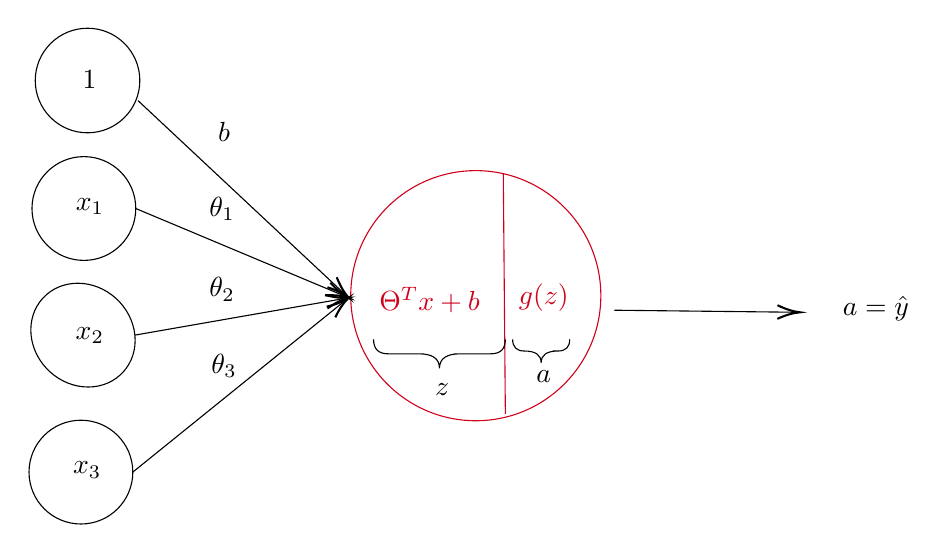
\begin{tikzpicture}[x=0.75pt,y=0.75pt,yscale=-1,xscale=1]
%uncomment if require: \path (0,300); %set diagram left start at 0, and has height of 300

%Shape: Circle [id:dp4894456216466021] 
\draw   (73.43,102) .. controls (73.43,88.19) and (84.63,77) .. (98.43,77) .. controls (112.24,77) and (123.43,88.19) .. (123.43,102) .. controls (123.43,115.81) and (112.24,127) .. (98.43,127) .. controls (84.63,127) and (73.43,115.81) .. (73.43,102) -- cycle ;
%Shape: Circle [id:dp5135503842228779] 
\draw   (73,163) .. controls (71.62,149.19) and (81.69,138) .. (95.5,138) .. controls (109.31,138) and (121.62,149.19) .. (123,163) .. controls (124.38,176.81) and (114.31,188) .. (100.5,188) .. controls (86.69,188) and (74.38,176.81) .. (73,163) -- cycle ;
%Shape: Circle [id:dp5054751399658592] 
\draw   (72,229) .. controls (72,215.19) and (83.19,204) .. (97,204) .. controls (110.81,204) and (122,215.19) .. (122,229) .. controls (122,242.81) and (110.81,254) .. (97,254) .. controls (83.19,254) and (72,242.81) .. (72,229) -- cycle ;
%Shape: Circle [id:dp7068247835752886] 
\draw  [color={rgb, 255:red, 208; green, 2; blue, 27 }  ,draw opacity=1 ] (227,144) .. controls (227,110.72) and (253.97,83.75) .. (287.25,83.75) .. controls (320.53,83.75) and (347.5,110.72) .. (347.5,144) .. controls (347.5,177.28) and (320.53,204.25) .. (287.25,204.25) .. controls (253.97,204.25) and (227,177.28) .. (227,144) -- cycle ;
%Straight Lines [id:da3951259360286594] 
\draw    (123.43,102) -- (224.16,144.23) ;
\draw [shift={(226,145)}, rotate = 202.75] [color={rgb, 255:red, 0; green, 0; blue, 0 }  ][line width=0.75]    (10.93,-3.29) .. controls (6.95,-1.4) and (3.31,-0.3) .. (0,0) .. controls (3.31,0.3) and (6.95,1.4) .. (10.93,3.29)   ;

%Straight Lines [id:da17712089576257095] 
\draw    (123,163) -- (224.03,145.34) ;
\draw [shift={(226,145)}, rotate = 530.0899999999999] [color={rgb, 255:red, 0; green, 0; blue, 0 }  ][line width=0.75]    (10.93,-3.29) .. controls (6.95,-1.4) and (3.31,-0.3) .. (0,0) .. controls (3.31,0.3) and (6.95,1.4) .. (10.93,3.29)   ;

%Straight Lines [id:da10379609280096158] 
\draw    (122,229) -- (224.44,146.26) ;
\draw [shift={(226,145)}, rotate = 501.07] [color={rgb, 255:red, 0; green, 0; blue, 0 }  ][line width=0.75]    (10.93,-3.29) .. controls (6.95,-1.4) and (3.31,-0.3) .. (0,0) .. controls (3.31,0.3) and (6.95,1.4) .. (10.93,3.29)   ;

%Straight Lines [id:da1555895906794451] 
\draw    (354,151) -- (441.5,151.98) ;
\draw [shift={(443.5,152)}, rotate = 180.64] [color={rgb, 255:red, 0; green, 0; blue, 0 }  ][line width=0.75]    (10.93,-3.29) .. controls (6.95,-1.4) and (3.31,-0.3) .. (0,0) .. controls (3.31,0.3) and (6.95,1.4) .. (10.93,3.29)   ;

%Shape: Circle [id:dp07492513539205437] 
\draw   (75,40.33) .. controls (75,26.42) and (86.28,15.14) .. (100.19,15.14) .. controls (114.1,15.14) and (125.38,26.42) .. (125.38,40.33) .. controls (125.38,54.24) and (114.1,65.52) .. (100.19,65.52) .. controls (86.28,65.52) and (75,54.24) .. (75,40.33) -- cycle ;
%Straight Lines [id:da37710728737628485] 
\draw    (124.5,50) -- (224.54,143.63) ;
\draw [shift={(226,145)}, rotate = 223.11] [color={rgb, 255:red, 0; green, 0; blue, 0 }  ][line width=0.75]    (10.93,-3.29) .. controls (6.95,-1.4) and (3.31,-0.3) .. (0,0) .. controls (3.31,0.3) and (6.95,1.4) .. (10.93,3.29)   ;

%Straight Lines [id:da9942335357246543] 
\draw [color={rgb, 255:red, 208; green, 2; blue, 27 }  ,draw opacity=1 ]   (300.5,85) -- (301.5,201) ;


%Shape: Brace [id:dp48208896309529936] 
\draw   (238,165) .. controls (238,169.67) and (240.33,172) .. (245,172) -- (259.75,172) .. controls (266.42,172) and (269.75,174.33) .. (269.75,179) .. controls (269.75,174.33) and (273.08,172) .. (279.75,172)(276.75,172) -- (294.5,172) .. controls (299.17,172) and (301.5,169.67) .. (301.5,165) ;
%Shape: Brace [id:dp308784031815875] 
\draw   (305,165) .. controls (305,168.77) and (306.89,170.66) .. (310.66,170.66) -- (310.66,170.66) .. controls (316.05,170.66) and (318.75,172.55) .. (318.75,176.32) .. controls (318.75,172.55) and (321.45,170.66) .. (326.84,170.66)(324.41,170.66) -- (326.84,170.66) .. controls (330.61,170.66) and (332.5,168.77) .. (332.5,165) ;

% Text Node
\draw (101.3,163) node   {$x_{2}$};
% Text Node
\draw (101.37,100.96) node   {$x_{1}$};
% Text Node
\draw (100,228) node   {$x_{3}$};
% Text Node
\draw (101.21,39.84) node   {$1$};
% Text Node
\draw (166,65) node   {$b$};
% Text Node
\draw (165,102) node   {$\theta _{1}$};
% Text Node
\draw (165,141) node   {$\theta _{2}$};
% Text Node
\draw (166,178) node   {$\theta _{3}$};
% Text Node
\draw (480,150) node   {$a=\hat{y}$};
% Text Node
\draw (320,145) node [color={rgb, 255:red, 208; green, 2; blue, 27 }  ,opacity=1 ]  {$g( z)$};
% Text Node
\draw (265,146) node [color={rgb, 255:red, 208; green, 2; blue, 27 }  ,opacity=1 ]  {$\Theta ^{T} x+b$};
% Text Node
\draw (271,189) node   {$z$};
% Text Node
\draw (320,183) node   {$a$};


\end{tikzpicture}


}
\caption{Single layer neural network. The input $x$ is multiplied by the weights $w$ to be passed to the neuron and generate the output $\hat { y }$~\brackettext{\cite{AndrewNgDL}}.}
\label{fig:preceptron}
\end{figure}
A single neuron is shown in Figure~\ref{fig:preceptron}. The computational unit illustrated in red takes in the different features $x$ and multiplies each input with a given weight $w$. The weights indicate the importance of each feature for the computation. The neuron then performs a non-linear transformation to the input and generates the output ($\hat { y } $). $b$ is called the \emph{bias unit} which always has as input value of $1$. $g(x)$ is called the \emph{activation
function} and represents the non-linear transformation that is applied on the input data. Essentially, each neuron consists of two steps of computation. First, $z$ is computed by the multiplication of weights and inputs. Second, an activation function of choice is applied to $z$ to produce the final output. The output or activation ($a$) of the last unit is the predicted output. A neural network is a group of different neurons connected together, as shown in Figure~\ref{fig:nn}. In a
neural network, the first layer is called the input layer and the last layer is called the output layer. Any layer in between is considered as a hidden layer. Typically, the values of the input and the output layer are given in the training set. Activation of each computational unit is the output of that unit after applying a certain function on the inputs, we denote activation of unit (neuron) $i$ in layer $j$ by $a_{i}^{[j]}$. The $w^{(j)}_{nl}$ is the weight controlling the function mapping from layer $j$ to layer $j+1$ between unit $n$ in layer $j$ and $l$ in $j+1$. Learning this weight matrix is the final goal of any deep learning system. The weights indicate how different features of inputs should be combined and how much should each of them influence the final output. The values of intermediate activations can be interpreted as latent features discovered during training. Features are combined with new weights to either generate an intermediate or a final
result~\brackettext{\cite{ng2000cs229,haykin2009neural}}. \\
\begin{figure}
\centering 
\resizebox{0.65\textwidth}{0.4\textwidth}{      
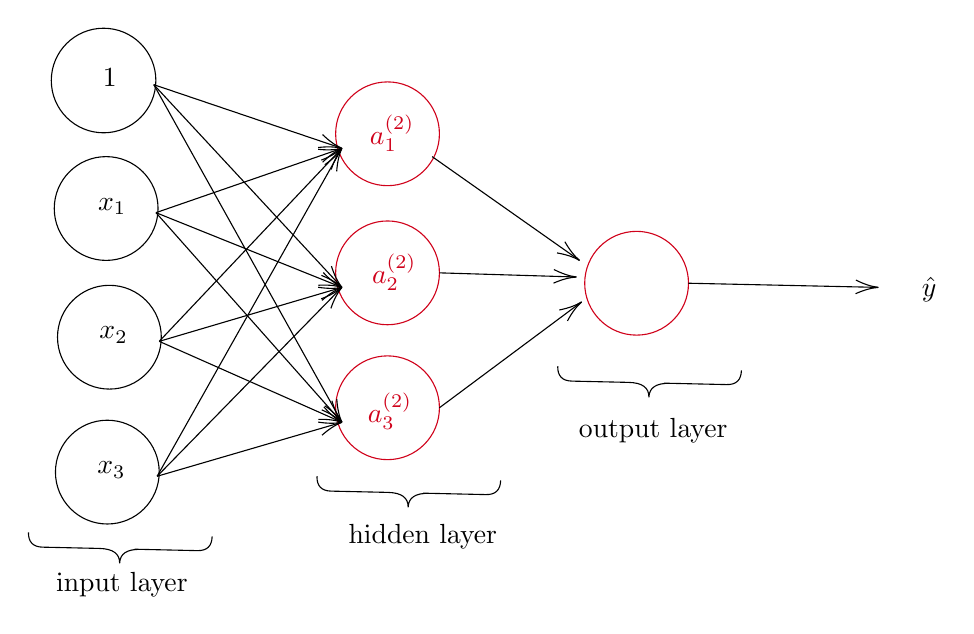
\begin{tikzpicture}[x=0.75pt,y=0.75pt,yscale=-1,xscale=1]
%uncomment if require: \path (0,300); %set diagram left start at 0, and has height of 300

\draw  [color={rgb, 255:red, 208; green, 2; blue, 27 }  ,draw opacity=1 ]  (241, 71) circle [x radius= 25, y radius= 25]  ;
\draw  [color={rgb, 255:red, 208; green, 2; blue, 27 }  ,draw opacity=1 ]  (241, 138) circle [x radius= 25, y radius= 25]  ;
\draw  [color={rgb, 255:red, 208; green, 2; blue, 27 }  ,draw opacity=1 ]  (241, 203) circle [x radius= 25, y radius= 25]  ;
\draw    (262.5,82) -- (333.5,132) ;
\draw [shift={(333.5,132)}, rotate = 215.15] [color={rgb, 255:red, 0; green, 0; blue, 0 }  ]   (0,0) .. controls (3.31,-0.3) and (6.95,-1.4) .. (10.93,-3.29)(0,0) .. controls (3.31,0.3) and (6.95,1.4) .. (10.93,3.29)   ;

\draw    (266,138) -- (332,140) ;
\draw [shift={(332,140)}, rotate = 181.74] [color={rgb, 255:red, 0; green, 0; blue, 0 }  ]   (0,0) .. controls (3.31,-0.3) and (6.95,-1.4) .. (10.93,-3.29)(0,0) .. controls (3.31,0.3) and (6.95,1.4) .. (10.93,3.29)   ;

\draw    (266,203) -- (334.5,152) ;
\draw [shift={(334.5,152)}, rotate = 503.33] [color={rgb, 255:red, 0; green, 0; blue, 0 }  ]   (0,0) .. controls (3.31,-0.3) and (6.95,-1.4) .. (10.93,-3.29)(0,0) .. controls (3.31,0.3) and (6.95,1.4) .. (10.93,3.29)   ;

\draw  [color={rgb, 255:red, 208; green, 2; blue, 27 }  ,draw opacity=1 ]  (361, 143) circle [x radius= 25, y radius= 25]  ;
\draw    (386,143) -- (477.5,145) ;
\draw [shift={(477.5,145)}, rotate = 181.25] [color={rgb, 255:red, 0; green, 0; blue, 0 }  ]   (0,0) .. controls (3.31,-0.3) and (6.95,-1.4) .. (10.93,-3.29)(0,0) .. controls (3.31,0.3) and (6.95,1.4) .. (10.93,3.29)   ;

\draw    (105.43, 107) circle [x radius= 25, y radius= 25]  ;
\draw    (107, 169) circle [x radius= 25, y radius= 25]  ;
\draw    (106, 234) circle [x radius= 25, y radius= 25]  ;
\draw    (104.19, 45.33) circle [x radius= 25.19, y radius= 25.19]  ;
\draw    (128.38,47.33) -- (219,78) ;
\draw [shift={(219,78)}, rotate = 198.7] [color={rgb, 255:red, 0; green, 0; blue, 0 }  ]   (0,0) .. controls (3.31,-0.3) and (6.95,-1.4) .. (10.93,-3.29)(0,0) .. controls (3.31,0.3) and (6.95,1.4) .. (10.93,3.29)   ;

\draw    (128.38,47.33) -- (219,145) ;
\draw [shift={(219,145)}, rotate = 227.14] [color={rgb, 255:red, 0; green, 0; blue, 0 }  ]   (0,0) .. controls (3.31,-0.3) and (6.95,-1.4) .. (10.93,-3.29)(0,0) .. controls (3.31,0.3) and (6.95,1.4) .. (10.93,3.29)   ;

\draw    (128.38,47.33) -- (219,210) ;
\draw [shift={(219,210)}, rotate = 240.88] [color={rgb, 255:red, 0; green, 0; blue, 0 }  ]   (0,0) .. controls (3.31,-0.3) and (6.95,-1.4) .. (10.93,-3.29)(0,0) .. controls (3.31,0.3) and (6.95,1.4) .. (10.93,3.29)   ;

\draw    (129.43,109) -- (219,210) ;
\draw [shift={(219,210)}, rotate = 228.43] [color={rgb, 255:red, 0; green, 0; blue, 0 }  ]   (0,0) .. controls (3.31,-0.3) and (6.95,-1.4) .. (10.93,-3.29)(0,0) .. controls (3.31,0.3) and (6.95,1.4) .. (10.93,3.29)   ;

\draw    (129.43,109) -- (219,145) ;
\draw [shift={(219,145)}, rotate = 201.9] [color={rgb, 255:red, 0; green, 0; blue, 0 }  ]   (0,0) .. controls (3.31,-0.3) and (6.95,-1.4) .. (10.93,-3.29)(0,0) .. controls (3.31,0.3) and (6.95,1.4) .. (10.93,3.29)   ;

\draw    (129.43,109) -- (219,78) ;
\draw [shift={(219,78)}, rotate = 520.9100000000001] [color={rgb, 255:red, 0; green, 0; blue, 0 }  ]   (0,0) .. controls (3.31,-0.3) and (6.95,-1.4) .. (10.93,-3.29)(0,0) .. controls (3.31,0.3) and (6.95,1.4) .. (10.93,3.29)   ;

\draw    (131,171) -- (219,78) ;
\draw [shift={(219,78)}, rotate = 493.42] [color={rgb, 255:red, 0; green, 0; blue, 0 }  ]   (0,0) .. controls (3.31,-0.3) and (6.95,-1.4) .. (10.93,-3.29)(0,0) .. controls (3.31,0.3) and (6.95,1.4) .. (10.93,3.29)   ;

\draw    (131,171) -- (219,145) ;
\draw [shift={(219,145)}, rotate = 523.54] [color={rgb, 255:red, 0; green, 0; blue, 0 }  ]   (0,0) .. controls (3.31,-0.3) and (6.95,-1.4) .. (10.93,-3.29)(0,0) .. controls (3.31,0.3) and (6.95,1.4) .. (10.93,3.29)   ;

\draw    (131,171) -- (219,210) ;
\draw [shift={(219,210)}, rotate = 203.9] [color={rgb, 255:red, 0; green, 0; blue, 0 }  ]   (0,0) .. controls (3.31,-0.3) and (6.95,-1.4) .. (10.93,-3.29)(0,0) .. controls (3.31,0.3) and (6.95,1.4) .. (10.93,3.29)   ;

\draw    (130,236) -- (219,78) ;
\draw [shift={(219,78)}, rotate = 479.39] [color={rgb, 255:red, 0; green, 0; blue, 0 }  ]   (0,0) .. controls (3.31,-0.3) and (6.95,-1.4) .. (10.93,-3.29)(0,0) .. controls (3.31,0.3) and (6.95,1.4) .. (10.93,3.29)   ;

\draw    (130,236) -- (219,145) ;
\draw [shift={(219,145)}, rotate = 494.36] [color={rgb, 255:red, 0; green, 0; blue, 0 }  ]   (0,0) .. controls (3.31,-0.3) and (6.95,-1.4) .. (10.93,-3.29)(0,0) .. controls (3.31,0.3) and (6.95,1.4) .. (10.93,3.29)   ;

\draw    (130,236) -- (219,210) ;
\draw [shift={(219,210)}, rotate = 523.72] [color={rgb, 255:red, 0; green, 0; blue, 0 }  ]   (0,0) .. controls (3.31,-0.3) and (6.95,-1.4) .. (10.93,-3.29)(0,0) .. controls (3.31,0.3) and (6.95,1.4) .. (10.93,3.29)   ;

\draw   (68,263) .. controls (67.89,267.67) and (70.17,270.05) .. (74.84,270.16) -- (102.1,270.77) .. controls (108.76,270.92) and (112.04,273.32) .. (111.93,277.99) .. controls (112.04,273.32) and (115.42,271.07) .. (122.09,271.22)(119.09,271.15) -- (149.34,271.83) .. controls (154.01,271.94) and (156.39,269.66) .. (156.5,264.99) ;
\draw   (207,236) .. controls (206.89,240.67) and (209.17,243.05) .. (213.84,243.16) -- (241.1,243.77) .. controls (247.76,243.92) and (251.04,246.32) .. (250.93,250.99) .. controls (251.04,246.32) and (254.42,244.07) .. (261.09,244.22)(258.09,244.15) -- (288.34,244.83) .. controls (293.01,244.94) and (295.39,242.66) .. (295.5,237.99) ;
\draw   (323,183) .. controls (322.89,187.67) and (325.17,190.05) .. (329.84,190.16) -- (357.1,190.77) .. controls (363.76,190.92) and (367.04,193.32) .. (366.93,197.99) .. controls (367.04,193.32) and (370.42,191.07) .. (377.09,191.22)(374.09,191.15) -- (404.34,191.83) .. controls (409.01,191.94) and (411.39,189.66) .. (411.5,184.99) ;

\draw (243.21,70.84) node [color={rgb, 255:red, 208; green, 2; blue, 27 }  ,opacity=1 ]  {$a^{( 2)}_{1}$};
\draw (244.21,137.84) node [color={rgb, 255:red, 208; green, 2; blue, 27 }  ,opacity=1 ]  {$a^{( 2)}_{2}$};
\draw (242.21,204.84) node [color={rgb, 255:red, 208; green, 2; blue, 27 }  ,opacity=1 ]  {$a^{( 2)}_{3}$};
\draw (109,168) node   {$x_{2}$};
\draw (108.37,105.96) node   {$x_{1}$};
\draw (108,233) node   {$x_{3}$};
\draw (107.21,43.84) node   {$1$};
\draw (502,146) node   {$\hat{y}$};
\draw (113,288) node   {input layer};
\draw (258,265) node   {hidden layer};
\draw (369,214) node   {output layer};


\end{tikzpicture}

}
    \caption{Two layer neural network with one hidden layer (input layer is layer-$0$). Input $x$ is multiplied by the weights $w$ to generate intermediate activation $a$. The output $\hat { y } $ is the combination of activations with their weights~\brackettext{\cite{AndrewNgML}}.}
\label{fig:nn}
\end{figure}
\noindent
There are different classes of activation functions available but the most commonly used ones are \emph{Sigmoid} and \emph{Relu}, illustrated in Figure~\ref{fig:activation}. An example of forward computation of the network in Figure~\ref{fig:nn} is given in Equation~\ref{eq:nn_eq}. Although a single output is shown in both figures, the output layer can have different sizes. It can vary from one output for a single class classification to $10$ for a multi-class classification with $10$ classes and even in some cases $10,000$ pixels of a image. How different neurons connect, the choice of activation function, the shape of the output layer and the number of layers is what defines different architectures. In the following, we only consider the architecture needed to generate word embeddings. 
\begin{equation}
\begin{split}
a_{ 1 }^{ [2] }=g(w _{ 10 }^{ [1] }x_{ 0 }+w _{ 11 }^{ [1]}x_{ 1 }+w _{ 12 }^{ [1] }x_{ 2 }+w _{ 13 }^{ [1] }x_{ 3 })\\ 
a_{ 2 }^{ [2] }=g(w _{ 20 }^{ 1] }x_{ 0 }+w _{ 21 }^{ 1] }x_{ 1 }+w _{ 22 }^{ [1] }x_{ 2 }+w _{ 23 }^{ (1) }x_{ 3 })\\
 a_{ 3 }^{ [2] }=g(w _{ 30 }^{ [1] }x_{ 0 }+w _{ 31 }^{ 1] }x_{ 1 }+w _{ 32 }^{ [1] }x_{ 2 }+w _{ 33 }^{ 1] }x_{ 3 })\\
  \hat { y } =a_{ 1 }^{ [3] }=g(w _{ 10 }^{ [2] }x_{ 0 }+w _{ 11 }^{ [2] }x_{ 1 }+w _{ 12 }^{ [2] }x_{ 2 }+w _{ 13 }^{ [2] }x_{ 3 })
\end{split}
\label{eq:nn_eq}
\end{equation}


\begin{figure}
\centering
\subcaptionbox{\label{sfig:relu}}{\includegraphics[width=0.45\linewidth , height=0.30\linewidth]{images/relu.png}}
\subcaptionbox{\label{sfig:sigmoid}}{\includegraphics[width=0.45\linewidth , height=0.30\linewidth]{images/sigmoid.png}}
\caption{Common choices of activation functions:~\subref{sfig:relu} Relu function $a=max(0,x)$ (simply cutting values below zero) and ~\subref{sfig:sigmoid} Sigmoid function $a=\frac{1}{1+e^{x}}$, which forces the values to be between zero and one.}
\label{fig:activation}
\end{figure}
\subsection{Training  Neural networks}
Consider the output $\hat { y } $ as the prediction of our network for some task. In a supervised learning problem the aim is to reduce the error between the prediction ($\hat { y } $) and the true label $y$. As a result the cost function can be defined as $J$ in Equation~\ref{eq:cost_nn}, where $L$ denotes the loss function on a single training example and $m$ is the size of the training set. The cost function is simply the sum of all losses on the training set.
\begin{equation}
J(w,b)=\sum _{ j=1 }^{ m }{ L( } \hat { y }^{ (i) } ,y^{ (i) })
\label{eq:cost_nn}
\end{equation}
The goal of the training phase is to learn $w$ and $b$ such that the overall cost is minimized. \\
\noindent 
One method to solve this optimization problem is called \emph{Gradient Descent} (GD)~\brackettext{\cite{DBLP:journals/corr/Ruder16}}. Considering the most simple case (a function with only one parameter) the gradient descent is illustrated in Figure~\ref{fig:gradientD}. Gradient descent is a way to minimize an objective function parameterized by a model’s parameters by updating the parameters in the opposite direction of the gradient w.r.t. to the parameters. The algorithm for one parameter $w$ can be
seen in Algorithm~\ref{algo:gd}, $\alpha$ is the \emph{learning rate} or the step size and shows how big a step is we take in each iteration. As shown in Figure~\ref{fig:gradientD} the derivative or the slope of the function is positive on the right side of the minimum (the update rule will decrease $w$) and negative on the left size (the update rule will increase $w$). \\


\begin{algorithm}[htbp]
  %
  \begin{algorithmic}[1]
    \newcommand{\UF}{\mathrm{U}}
   \While{(not converged)}
 \State $w=: w- \alpha\frac { \partial J(w) }{ \partial w } $
  \EndWhile
  \end{algorithmic}
  %
\caption{:Gradient decent }
 \label{algo:gd}
\end{algorithm}

\begin{figure}
\centering 
\resizebox{0.65\textwidth}{0.4\textwidth}{      
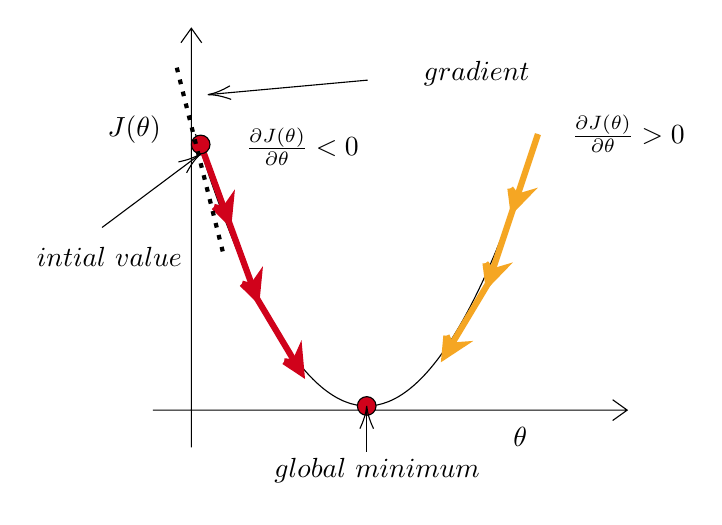
\begin{tikzpicture}[x=0.75pt,y=0.75pt,yscale=-1,xscale=1]
%uncomment if require: \path (0,300); %set diagram left start at 0, and has height of 300

\draw  (75,190) -- (303.5,190)(93.5,6) -- (93.5,208) (296.5,185) -- (303.5,190) -- (296.5,195) (88.5,13) -- (93.5,6) -- (98.5,13)  ;
\draw   (95.5,57) .. controls (150.5,231.67) and (205.5,231.67) .. (260.5,57) ;
\draw [color={rgb, 255:red, 208; green, 2; blue, 27 }  ,draw opacity=1 ][line width=2.25]    (98,62) -- (111.5,99) ;
\draw [shift={(111.5,99)}, rotate = 249.95] [color={rgb, 255:red, 208; green, 2; blue, 27 }  ,draw opacity=1 ][fill={rgb, 255:red, 208; green, 2; blue, 27 }  ,fill opacity=1 ][line width=2.25]   (8.93,-4.29) -- (0,0) -- (8.93,4.29) -- (5.93,0) -- (8.93,-4.29)    ;

\draw [color={rgb, 255:red, 208; green, 2; blue, 27 }  ,draw opacity=1 ][line width=2.25]    (111.5,99) -- (125,136) ;
\draw [shift={(125,136)}, rotate = 249.95] [color={rgb, 255:red, 208; green, 2; blue, 27 }  ,draw opacity=1 ][fill={rgb, 255:red, 208; green, 2; blue, 27 }  ,fill opacity=1 ][line width=2.25]   (8.93,-4.29) -- (0,0) -- (8.93,4.29) -- (5.93,0) -- (8.93,-4.29)    ;

\draw [color={rgb, 255:red, 208; green, 2; blue, 27 }  ,draw opacity=1 ][line width=2.25]    (125,136) -- (146.5,172) ;
\draw [shift={(146.5,172)}, rotate = 239.15] [color={rgb, 255:red, 208; green, 2; blue, 27 }  ,draw opacity=1 ][fill={rgb, 255:red, 208; green, 2; blue, 27 }  ,fill opacity=1 ][line width=2.25]   (8.93,-4.29) -- (0,0) -- (8.93,4.29) -- (5.93,0) -- (8.93,-4.29)    ;

\draw [color={rgb, 255:red, 245; green, 166; blue, 35 }  ,draw opacity=1 ][line width=2.25]    (260.5,57) -- (248.5,93) ;
\draw [shift={(248.5,93)}, rotate = 288.43] [color={rgb, 255:red, 245; green, 166; blue, 35 }  ,draw opacity=1 ][fill={rgb, 255:red, 245; green, 166; blue, 35 }  ,fill opacity=1 ][line width=2.25]   (8.93,-4.29) -- (0,0) -- (8.93,4.29) -- (5.93,0) -- (8.93,-4.29)    ;

\draw [color={rgb, 255:red, 245; green, 166; blue, 35 }  ,draw opacity=1 ][line width=2.25]    (248.5,93) -- (236.5,129) ;
\draw [shift={(236.5,129)}, rotate = 288.43] [color={rgb, 255:red, 245; green, 166; blue, 35 }  ,draw opacity=1 ][fill={rgb, 255:red, 245; green, 166; blue, 35 }  ,fill opacity=1 ][line width=2.25]   (8.93,-4.29) -- (0,0) -- (8.93,4.29) -- (5.93,0) -- (8.93,-4.29)    ;

\draw [color={rgb, 255:red, 245; green, 166; blue, 35 }  ,draw opacity=1 ][line width=2.25]    (236.5,129) -- (215.5,164) ;
\draw [shift={(215.5,164)}, rotate = 300.96] [color={rgb, 255:red, 245; green, 166; blue, 35 }  ,draw opacity=1 ][fill={rgb, 255:red, 245; green, 166; blue, 35 }  ,fill opacity=1 ][line width=2.25]   (8.93,-4.29) -- (0,0) -- (8.93,4.29) -- (5.93,0) -- (8.93,-4.29)    ;

\draw  [fill={rgb, 255:red, 208; green, 2; blue, 27 }  ,fill opacity=1 ]  (98, 62) circle [x radius= 4.5, y radius= 4.5]  ;
\draw    (50.5,102) -- (98,66.5) ;
\draw [shift={(98,66.5)}, rotate = 503.23] [color={rgb, 255:red, 0; green, 0; blue, 0 }  ]   (0,0) .. controls (3.31,-0.3) and (6.95,-1.4) .. (10.93,-3.29)(0,0) .. controls (3.31,0.3) and (6.95,1.4) .. (10.93,3.29)   ;

\draw  [fill={rgb, 255:red, 208; green, 2; blue, 27 }  ,fill opacity=1 ]  (178, 188) circle [x radius= 4.5, y radius= 4.5]  ;
\draw    (178,210) -- (178,188) ;
\draw [shift={(178,188)}, rotate = 450] [color={rgb, 255:red, 0; green, 0; blue, 0 }  ]   (0,0) .. controls (3.31,-0.3) and (6.95,-1.4) .. (10.93,-3.29)(0,0) .. controls (3.31,0.3) and (6.95,1.4) .. (10.93,3.29)   ;

\draw [line width=1.5]  [dash pattern={on 1.69pt off 2.76pt}]  (86.5,25) -- (109.5,117) ;


\draw    (178.5,31) -- (101.5,38) ;
\draw [shift={(101.5,38)}, rotate = 354.81] [color={rgb, 255:red, 0; green, 0; blue, 0 }  ]   (0,0) .. controls (3.31,-0.3) and (6.95,-1.4) .. (10.93,-3.29)(0,0) .. controls (3.31,0.3) and (6.95,1.4) .. (10.93,3.29)   ;


\draw (252,203) node   {$\theta$};
\draw (66,55) node   {$J( \theta)$};
\draw (147,63) node   {$\frac{\partial J(\theta)}{\partial \theta} < 0$};
\draw (304,57) node   {$\frac{\partial J(\theta)}{\partial \theta}  >0$};
\draw (183,219) node   {$global\ minimum$};
\draw (54,116) node   {$intial\ value$};
\draw (231,28) node   {$gradient$};


\end{tikzpicture}

}
\caption{Gradient decent on a function with only one parameter. In each iteration, we take a step in the direction of the gradient. The gradient will guide the algorithm to the functions minimum. }
\label{fig:gradientD}
\end{figure}
\noindent
In a dataset with $m$ training examples, for each training example, the gradient of the cost function with respect to every weight and bias has to be calculated and accumulated. After iterating through all the training examples the weights and bias term will be updated according to Algorithm~\ref{algo:gd}. This process is repeated from start to finish for some number of iterations. There exist three variations of~GD: 
\begin{itemize}
\item \textbf{Mini-batch GD: } Instead of iterating over all training examples, a subset of a batch is considered, before making an update. This is a good choice for very large datasets.
\item \textbf{Stochastic-GD: } In this case, only one example is looked at, before making an update. 
\item \textbf{Batch-GD: } The original algorithm with iteration over all examples. 
\end{itemize}

\subsection{Word embeddings}\label{subsec:wordembeddings}
One of the challenges of machine learning is to come up with valuable features for algorithms. These feature often have to be task specific and reflect the needs of the downstream tasks. \emph{Representation learning} attempts to learn good features and representations automatically \cite{DBLP:journals/corr/ZhongWD16}. PCA is one example of traditional methods for learning low-dimensional representation from high dimensional data. In a deep learning architecture, the output of each intermediate layer can be viewed as a representation of the original input data. As illustrated in Figure~\ref{fig:preceptron} each unit of the network computes a non-linear combination of the inputs which is used by the next layer. If the dimension of the hidden layer is much smaller than the input layer, a low dimensional representation of the data is learned in the hidden layer. Word embeddings use this attribute to learn dense vector representation for each word in the text.\\
\noindent
Text is inherently high dimensional. In most traditional NLP systems, each word is denoted by a one-hot vector~\footnote{binary vector in the size of the vocabulary that has value of one on the index of the word it refers to and zero in all other indexes.} in the size of the vocabulary, which was not only sparse but high dimensional. By feeding these high dimensional representations to a neural network with a smaller hidden layer, a new representation (usually in the order of $100$ dimensions) of each word can be learned. Although neural networks can be used in supervised and unsupervised learning, generally, the embedding is
learned to form a supervised learning problem. For this purpose, different models have been proposed, the most famous being word2vec (explained briefly in chapter~\ref{chap:intro}). All the models follow the same principle illustrated in Figure~\ref{fig:emb}. The size of the output layer depends on the particular architecture and the cost function. In addition, the network can be multiple layers deep, but for our purposes, we focus on shallow networks with only one hidden layer. Most of the well-established methods tend to focus on capturing meaningful relations between words with similar meaning and little work has been done to make the embedding match to a certain task. The facetted embedding model proposed in the next chapter tries to solve this problem by adding the extra entity-type information. The model, if work as expected, will be more useful in information retrieval and exploration of news streams than other embedding methods. In the next section, we will discuss GloVe, which is the basis for the facetted embedding model.
\begin{figure}
\centering 
\resizebox{0.8\textwidth}{0.5\textwidth}{      
\begin{tikzpicture}[x=0.75pt,y=0.75pt,yscale=-1,xscale=1]
%uncomment if require: \path (0,406); %set diagram left start at 0, and has height of 406

\draw  [color={rgb, 255:red, 208; green, 2; blue, 27 }  ,draw opacity=1 ]  (302, 69) circle [x radius= 25, y radius= 25]  ;
\draw  [color={rgb, 255:red, 208; green, 2; blue, 27 }  ,draw opacity=1 ]  (301, 135) circle [x radius= 25, y radius= 25]  ;
\draw  [color={rgb, 255:red, 208; green, 2; blue, 27 }  ,draw opacity=1 ]  (301, 200) circle [x radius= 25, y radius= 25]  ;
\draw    (322.5,79) -- (411.5,133) ;
\draw [shift={(411.5,133)}, rotate = 211.25] [color={rgb, 255:red, 0; green, 0; blue, 0 }  ]   (0,0) .. controls (3.31,-0.3) and (6.95,-1.4) .. (10.93,-3.29)(0,0) .. controls (3.31,0.3) and (6.95,1.4) .. (10.93,3.29)   ;

\draw    (326,135) -- (411.5,133) ;
\draw [shift={(411.5,133)}, rotate = 538.6600000000001] [color={rgb, 255:red, 0; green, 0; blue, 0 }  ]   (0,0) .. controls (3.31,-0.3) and (6.95,-1.4) .. (10.93,-3.29)(0,0) .. controls (3.31,0.3) and (6.95,1.4) .. (10.93,3.29)   ;

\draw    (326,200) -- (411.5,133) ;
\draw [shift={(411.5,133)}, rotate = 501.92] [color={rgb, 255:red, 0; green, 0; blue, 0 }  ]   (0,0) .. controls (3.31,-0.3) and (6.95,-1.4) .. (10.93,-3.29)(0,0) .. controls (3.31,0.3) and (6.95,1.4) .. (10.93,3.29)   ;

\draw  [color={rgb, 255:red, 208; green, 2; blue, 27 }  ,draw opacity=1 ]  (433, 69) circle [x radius= 25, y radius= 25]  ;
\draw    (477.5,183) -- (551.5,183) ;
\draw [shift={(551.5,183)}, rotate = 180] [color={rgb, 255:red, 0; green, 0; blue, 0 }  ]   (0,0) .. controls (3.31,-0.3) and (6.95,-1.4) .. (10.93,-3.29)(0,0) .. controls (3.31,0.3) and (6.95,1.4) .. (10.93,3.29)   ;

\draw    (165.43, 104) circle [x radius= 25, y radius= 25]  ;
\draw    (168, 177) circle [x radius= 25, y radius= 25]  ;
\draw    (175, 256) circle [x radius= 25, y radius= 25]  ;
\draw    (164.19, 34.33) circle [x radius= 25.19, y radius= 25.19]  ;
\draw    (188.38,44.33) -- (279,75) ;
\draw [shift={(279,75)}, rotate = 198.7] [color={rgb, 255:red, 0; green, 0; blue, 0 }  ]   (0,0) .. controls (3.31,-0.3) and (6.95,-1.4) .. (10.93,-3.29)(0,0) .. controls (3.31,0.3) and (6.95,1.4) .. (10.93,3.29)   ;

\draw    (188.38,44.33) -- (279,142) ;
\draw [shift={(279,142)}, rotate = 227.14] [color={rgb, 255:red, 0; green, 0; blue, 0 }  ]   (0,0) .. controls (3.31,-0.3) and (6.95,-1.4) .. (10.93,-3.29)(0,0) .. controls (3.31,0.3) and (6.95,1.4) .. (10.93,3.29)   ;

\draw    (188.38,44.33) -- (279,207) ;
\draw [shift={(279,207)}, rotate = 240.88] [color={rgb, 255:red, 0; green, 0; blue, 0 }  ]   (0,0) .. controls (3.31,-0.3) and (6.95,-1.4) .. (10.93,-3.29)(0,0) .. controls (3.31,0.3) and (6.95,1.4) .. (10.93,3.29)   ;

\draw    (189.43,106) -- (279,207) ;
\draw [shift={(279,207)}, rotate = 228.43] [color={rgb, 255:red, 0; green, 0; blue, 0 }  ]   (0,0) .. controls (3.31,-0.3) and (6.95,-1.4) .. (10.93,-3.29)(0,0) .. controls (3.31,0.3) and (6.95,1.4) .. (10.93,3.29)   ;

\draw    (189.43,106) -- (279,142) ;
\draw [shift={(279,142)}, rotate = 201.9] [color={rgb, 255:red, 0; green, 0; blue, 0 }  ]   (0,0) .. controls (3.31,-0.3) and (6.95,-1.4) .. (10.93,-3.29)(0,0) .. controls (3.31,0.3) and (6.95,1.4) .. (10.93,3.29)   ;

\draw    (189.43,106) -- (279,75) ;
\draw [shift={(279,75)}, rotate = 520.9100000000001] [color={rgb, 255:red, 0; green, 0; blue, 0 }  ]   (0,0) .. controls (3.31,-0.3) and (6.95,-1.4) .. (10.93,-3.29)(0,0) .. controls (3.31,0.3) and (6.95,1.4) .. (10.93,3.29)   ;

\draw    (191,168) -- (279,75) ;
\draw [shift={(279,75)}, rotate = 493.42] [color={rgb, 255:red, 0; green, 0; blue, 0 }  ]   (0,0) .. controls (3.31,-0.3) and (6.95,-1.4) .. (10.93,-3.29)(0,0) .. controls (3.31,0.3) and (6.95,1.4) .. (10.93,3.29)   ;

\draw    (191,168) -- (279,142) ;
\draw [shift={(279,142)}, rotate = 523.54] [color={rgb, 255:red, 0; green, 0; blue, 0 }  ]   (0,0) .. controls (3.31,-0.3) and (6.95,-1.4) .. (10.93,-3.29)(0,0) .. controls (3.31,0.3) and (6.95,1.4) .. (10.93,3.29)   ;

\draw    (191,168) -- (279,207) ;
\draw [shift={(279,207)}, rotate = 203.9] [color={rgb, 255:red, 0; green, 0; blue, 0 }  ]   (0,0) .. controls (3.31,-0.3) and (6.95,-1.4) .. (10.93,-3.29)(0,0) .. controls (3.31,0.3) and (6.95,1.4) .. (10.93,3.29)   ;

\draw    (190,233) -- (279,75) ;
\draw [shift={(279,75)}, rotate = 479.39] [color={rgb, 255:red, 0; green, 0; blue, 0 }  ]   (0,0) .. controls (3.31,-0.3) and (6.95,-1.4) .. (10.93,-3.29)(0,0) .. controls (3.31,0.3) and (6.95,1.4) .. (10.93,3.29)   ;

\draw    (190,233) -- (279,142) ;
\draw [shift={(279,142)}, rotate = 494.36] [color={rgb, 255:red, 0; green, 0; blue, 0 }  ]   (0,0) .. controls (3.31,-0.3) and (6.95,-1.4) .. (10.93,-3.29)(0,0) .. controls (3.31,0.3) and (6.95,1.4) .. (10.93,3.29)   ;

\draw    (190,233) -- (279,207) ;
\draw [shift={(279,207)}, rotate = 523.72] [color={rgb, 255:red, 0; green, 0; blue, 0 }  ]   (0,0) .. controls (3.31,-0.3) and (6.95,-1.4) .. (10.93,-3.29)(0,0) .. controls (3.31,0.3) and (6.95,1.4) .. (10.93,3.29)   ;

\draw   (149.5,289) .. controls (149.5,293.67) and (151.83,296) .. (156.5,296) -- (172,296) .. controls (178.67,296) and (182,298.33) .. (182,303) .. controls (182,298.33) and (185.33,296) .. (192,296)(189,296) -- (207.5,296) .. controls (212.17,296) and (214.5,293.67) .. (214.5,289) ;
\draw   (267,233) .. controls (266.89,237.67) and (269.17,240.05) .. (273.84,240.16) -- (301.1,240.77) .. controls (307.76,240.92) and (311.04,243.32) .. (310.93,247.99) .. controls (311.04,243.32) and (314.42,241.07) .. (321.09,241.22)(318.09,241.15) -- (348.34,241.83) .. controls (353.01,241.94) and (355.39,239.66) .. (355.5,234.99) ;
\draw   (397,302) .. controls (396.89,306.67) and (399.17,309.05) .. (403.84,309.16) -- (431.1,309.77) .. controls (437.76,309.92) and (441.04,312.32) .. (440.93,316.99) .. controls (441.04,312.32) and (444.42,310.07) .. (451.09,310.22)(448.09,310.15) -- (478.34,310.83) .. controls (483.01,310.94) and (485.39,308.66) .. (485.5,303.99) ;
\draw    (7, 87) rectangle (137.5, 111.33)   ;
\draw    (7, 181) rectangle (137.5, 205.33)   ;
\draw    (8, 270) rectangle (138.5, 294.33)   ;
\draw  [color={rgb, 255:red, 208; green, 2; blue, 27 }  ,draw opacity=1 ]  (432, 143) circle [x radius= 25, y radius= 25]  ;
\draw  [color={rgb, 255:red, 208; green, 2; blue, 27 }  ,draw opacity=1 ]  (435, 207) circle [x radius= 25, y radius= 25]  ;
\draw  [color={rgb, 255:red, 208; green, 2; blue, 27 }  ,draw opacity=1 ]  (437, 272) circle [x radius= 25, y radius= 25]  ;
\draw    (326,135) -- (410,207) ;
\draw [shift={(410,207)}, rotate = 220.6] [color={rgb, 255:red, 0; green, 0; blue, 0 }  ]   (0,0) .. controls (3.31,-0.3) and (6.95,-1.4) .. (10.93,-3.29)(0,0) .. controls (3.31,0.3) and (6.95,1.4) .. (10.93,3.29)   ;

\draw    (322.5,79) -- (408,69) ;
\draw [shift={(408,69)}, rotate = 533.3299999999999] [color={rgb, 255:red, 0; green, 0; blue, 0 }  ]   (0,0) .. controls (3.31,-0.3) and (6.95,-1.4) .. (10.93,-3.29)(0,0) .. controls (3.31,0.3) and (6.95,1.4) .. (10.93,3.29)   ;

\draw    (322.5,79) -- (410,207) ;
\draw [shift={(410,207)}, rotate = 235.64] [color={rgb, 255:red, 0; green, 0; blue, 0 }  ]   (0,0) .. controls (3.31,-0.3) and (6.95,-1.4) .. (10.93,-3.29)(0,0) .. controls (3.31,0.3) and (6.95,1.4) .. (10.93,3.29)   ;

\draw    (322.5,79) -- (412,272) ;
\draw [shift={(412,272)}, rotate = 245.12] [color={rgb, 255:red, 0; green, 0; blue, 0 }  ]   (0,0) .. controls (3.31,-0.3) and (6.95,-1.4) .. (10.93,-3.29)(0,0) .. controls (3.31,0.3) and (6.95,1.4) .. (10.93,3.29)   ;

\draw    (326,135) -- (408,69) ;
\draw [shift={(408,69)}, rotate = 501.17] [color={rgb, 255:red, 0; green, 0; blue, 0 }  ]   (0,0) .. controls (3.31,-0.3) and (6.95,-1.4) .. (10.93,-3.29)(0,0) .. controls (3.31,0.3) and (6.95,1.4) .. (10.93,3.29)   ;

\draw    (326,200) -- (410,207) ;
\draw [shift={(410,207)}, rotate = 184.76] [color={rgb, 255:red, 0; green, 0; blue, 0 }  ]   (0,0) .. controls (3.31,-0.3) and (6.95,-1.4) .. (10.93,-3.29)(0,0) .. controls (3.31,0.3) and (6.95,1.4) .. (10.93,3.29)   ;

\draw    (326,200) -- (408,69) ;
\draw [shift={(408,69)}, rotate = 482.04] [color={rgb, 255:red, 0; green, 0; blue, 0 }  ]   (0,0) .. controls (3.31,-0.3) and (6.95,-1.4) .. (10.93,-3.29)(0,0) .. controls (3.31,0.3) and (6.95,1.4) .. (10.93,3.29)   ;

\draw    (328,200) -- (412,272) ;
\draw [shift={(412,272)}, rotate = 220.6] [color={rgb, 255:red, 0; green, 0; blue, 0 }  ]   (0,0) .. controls (3.31,-0.3) and (6.95,-1.4) .. (10.93,-3.29)(0,0) .. controls (3.31,0.3) and (6.95,1.4) .. (10.93,3.29)   ;

\draw    (326,135) -- (412,272) ;
\draw [shift={(412,272)}, rotate = 237.88] [color={rgb, 255:red, 0; green, 0; blue, 0 }  ]   (0,0) .. controls (3.31,-0.3) and (6.95,-1.4) .. (10.93,-3.29)(0,0) .. controls (3.31,0.3) and (6.95,1.4) .. (10.93,3.29)   ;


\draw (303.21,68.84) node [color={rgb, 255:red, 208; green, 2; blue, 27 }  ,opacity=1 ]  {$a^{( 2)}_{1}$};
\draw (305.21,136.84) node [color={rgb, 255:red, 208; green, 2; blue, 27 }  ,opacity=1 ]  {$a^{( 2)}_{2}$};
\draw (302.21,203.84) node [color={rgb, 255:red, 208; green, 2; blue, 27 }  ,opacity=1 ]  {$a^{( 2)}_{3}$};
\draw (169,178) node   {$x_{2}$};
\draw (168.37,102.96) node   {$x_{1}$};
\draw (175,256) node   {$x_{3}$};
\draw (167.21,32.84) node   {$1$};
\draw (578,186) node   {$\hat{y}$};
\draw (183,326) node   {$input\ layer$};
\draw (315,272) node   {$ \begin{gathered}
low\ dimensional\ \\
representation
\end{gathered}$};
\draw (444,335) node   {$output\ layer$};
\draw (72,99) node   {$0\ \ 0\ \ 0\ \ 0\ \ 0\ \ 0\ \ ..\ 0$};
\draw (13,77) node [rotate=-270]  {$a$};
\draw (29,60) node [rotate=-270]  {$brwon$};
\draw (46,63) node [rotate=-270]  {$dog$};
\draw (78,63) node [rotate=-270]  {$jumps$};
\draw (129,62) node [rotate=-270]  {$zoo$};
\draw (64,65) node [rotate=-270]  {$fox$};
\draw (72,193) node   {$0\ \ 0\ \ 0\ \ 1\ \ 0\ \ 0\ ..\ 0$};
\draw (13,171) node [rotate=-270]  {$a$};
\draw (29,154) node [rotate=-270]  {$brwon$};
\draw (46,157) node [rotate=-270]  {$dog$};
\draw (78,157) node [rotate=-270]  {$jumps$};
\draw (64,159) node [rotate=-270]  {$fox$};
\draw (73,282) node   {$0\ \ 0\ \ 0\ \ 0\ \ 0\ \ 0\ \ ..\ 0$};
\draw (14,260) node [rotate=-270]  {$a$};
\draw (30,243) node [rotate=-270]  {$brwon$};
\draw (47,246) node [rotate=-270]  {$dog$};
\draw (79,246) node [rotate=-270]  {$jumps$};
\draw (65,248) node [rotate=-270]  {$fox$};
\draw (125,159) node [rotate=-270]  {$zoo$};
\draw (130,246) node [rotate=-270]  {$zoo$};
\draw (110,64) node   {$...$};
\draw (108,160) node   {$...$};
\draw (111,248) node   {$...$};


\end{tikzpicture}

}
\caption{Underlying principle of word embeddings. The high dimensional one-hot vectors are the input of the network, through the hidden layer a dense representation is learned to either predict the surrounding words or optimize a different cost function in the output layer.}
\label{fig:emb}
\end{figure}
\section{Textual Based Embeddings }
\label{sec:textual}
Window-based models such as word2vec learn the embeddings in terms of a supervised learning task, where the objective is to predict a word's context given a center word in a fixed window. These models suffer from the disadvantage that they do not operate directly on the co-occurrence statistics of the corpus. Instead, they scan context windows across sentences, which fails to take advantage of the vast amount of repetition in the data. Regardless of the fact that many word co-occur together multiple time, for multiple pass through the data, a window-based method has to parse the whole corpus several times. Whereas, a co-occurrence matrix can capture this repetition in compact way and hence, save time and computational power.  \\
In contrast, matrix factorization methods operate directly on the co-occurrence matrix and capture the full statistics. Before, word2vec similar embeddings were generated using \emph{Singular Value Decomposition} (SVD) on co-occurrence matrices and keeping the top \emph{k} dimensions. These methods were also able to capture many semantic and syntactic analogies~\brackettext{\cite{Rohde06animproved}}. \brackettext{\cite{NIPS2014_5477}} showed that implicitly factorizing
a word-context matrix, whose cells are the \emph{Point-wise Mutual Information} (PMI) of
the respective word and context pairs, can generate embeddings close to word2vec. The main disadvantage of count based methods is that they are computationally slow on large matrices. In addition, adding new words to the model is difficult, since it requires training a new model from the start.\\
The \emph{GloVe}~\brackettext{\cite{DBLP:conf/emnlp/PenningtonSM14}} model combines the matrix factorization for generating embeddings with window-based methods and uses the global statistics of the corpus or in another word the co-occurrence matrix to generate embeddings. In addition, unlike the word2vec model that scales with the size of the corpus, general statistics of the data has to be generated only once in terms of the co-occurrence matrix and then additional computations can be performed on matrix alone.
\section{GloVe: Global Vector Embeddings}
\label{sec:GloVe}
The \emph{Global Vector Model} (GloVe) suggests that the ratio of co-occurrence probabilities can encode meaning components. An example can be seen in Table~\ref{table:tab_1}, in terms of studying a thermodynamic phase. A meaning component that sets the word  \emph{``ice''} apart from \emph{``steam''} can be represented as  a ratio of their occurrence probability with all other words \big($\frac { P(ice|k) }{ P(steam|k) } $, where $k$ can be any word in the vocabulary\big). This ratio is proved to better distinguish relevant words in comparison from irrelevant ones by giving the irrelevant ones a probability close to one. Also compared to the raw probabilities, it is better able to discriminate
between the relevant words by giving a high probability to a word like "solid" and low probability to \emph{``gas''}, making the word \emph{``ice'} stand out as a solid object. A word such as "\emph{``water''} or \emph{``fashion''} will, therefore, have a probability close to one as it is either a shared property or not related to the concept.\\
\begin{table}[]
\centering

\begin{tabular}{@{}l|l|l|l|l@{}}
\toprule
Probability and Ratio &  $k=solid$& $k=gas$ & $k=water$ &$k= fashion$  \\ \midrule $P(k|ice)$& {\color[HTML]{CB0000}large} &  {\color[HTML]{329A9D}small} & {\color[HTML]{CB0000}large} & {\color[HTML]{329A9D}small} \\\midrule
  $P(k|steam)$&{\color[HTML]{329A9D}small}  & {\color[HTML]{CB0000}large} &  {\color[HTML]{CB0000}large}&{\color[HTML]{329A9D}small}  \\\midrule
 $\frac { P(ice|k) }{ P(steam|k) } $& {\color[HTML]{CB0000}large} &  {\color[HTML]{329A9D}small}&  1 &    1  \\\midrule
\end{tabular}%
\caption{Co-occurrence probabilities for target words \emph{``ice'}and \emph{``steam'} with selected context words. Example taken from~\brackettext{\cite{DBLP:conf/emnlp/PenningtonSM14}}.}
\label{table:tab_1}
\end{table}

To capture these ratios, the authors of GloVe propose a log-bilinear model, where, if the dot product of two vectors corresponds to the log of their co-occurrence probability, their difference will show the meaning component, as seen in Equation~\ref{eq:log_prob}.

\begin{equation}
\begin{split}
\\ w_{ i }.w_{ j }=\log { P(i|j)\quad  } \\ w_{ x }(w_{ i }-w_{ j })=\log { \frac { P(x|j) }{ P(x|j) } \quad  } 
\end{split}
\label{eq:log_prob}
\end{equation}
Based on the log-bilinearity assumption, the cost function is defined as follows:\\
Let the matrix of word-word co-occurrence counts be denoted by $X\in { R }^{ V\times V }$, where $V$ is the size of the vocabulary. Entries $X_{ij}$ tabulate the number of times word $j$ occurs in the context of word $i$. $w_{ i }\in { R }^{ 1\times M }$ and $\tilde{w_{ j }}\in { R }^{ 1\times M }$ are the focal (center word) and context embeddings, respectively, where $M$ is the embedding size. The model tries to learn embeddings that minimize the squared difference between the dot product of the center word embedding and context embedding to the logarithm of its co-occurrence.  \\
Considering $ \tilde{b_{ j }}$ and $b_{ i }$  as the biases for the focal and context embeddings. The cost function is defined in Equation~\ref{eq:glove_cost}.  Since the log of co-occurrences does not directly result into a probability, in order to achieve the meaning component a normalization factor is needed. Bias $b_{ i }$ allows the model to learn this constant during training and $ \tilde{b_{ j }}$ is added to preserve symmetry. 
\begin{equation}
J=\sum _{ i,j=1 }^{ V }{ f({ X }_{ ij } } )(w_{ i }^{ T }\tilde{  w_{ j } } +b_{ i }+\tilde{  b_{ j } } -log{ X }_{ ij })^2
\label{eq:glove_cost}
\end{equation}
Optimizing for the co-occurrence counts alone might cause the model to be overwhelmed by the most common words. Therefore, function $f$ is introduced as a weighing function that imposes an upper bound on the maximum number of occurrences of a word. Conceptually,  $f$ scales the counts in order to avoid the influence of common words and boost the rare words. The choice of $f$ is not fixed but one class of functions that were used by the authors can be parametrized with $\alpha$ as the exponential weight and $x_{max}$ as the maximum number of allowed co-occurrences. $\alpha$ and $x_{max}$ are hyper-parameters that requires tuning, but the values suggested by the authors are for $\alpha$ is $\frac{3}{4}$ and for $x_{max}$ is $100$. 
\begin{equation}
f=\left\{
  \begin{array}{@{}ll@{}}
    (\frac { x }{ { x }_{ max } } )^{ \alpha  }& \text{if}\ x<x_{max} \\
    1 & \text{otherwise}
  \end{array}\right.
\label{eq:weighingfunction}
\end{equation}
\noindent
The model learns two embeddings for each word: one as a focal or center word and the other as a context word. As the co-occurrence matrix is symmetric both of which can be considered as learning the same representation. Ultimately, the two embeddings can be added to obtain the final embedding.
\section{LOAD: Implicit Network of Entities}
LOAD model is an entity co-occurrence graph representation of large document collections. For each document, named entities from sentences are extracted and connected based on their distance in a graph structure. The original LOAD model contains node types of pages and Sentences as well, which we disregard for the creation of facetted embeddings. \\
Equation~\ref{eq:load_dist} shows the weighing of a single edge in the LOAD model between two entities $v$ and $s$, where $\delta $ is a distance function. $\delta $ equals the number of sentences between the
instances, or $0$ if they occur in the same sentence. If $i$ and$ j$
do not occur on the same page: $ \delta(i, j) := \inf$. $ I_{ v }$ and $I_{ s } $ are the set of all instances of $v$ and $s$ in the corpus. $exp$ forces the weight to diminish exponentially with the distance. Eventually, the sum of all these exponential distances creates the final weight. 
\begin{equation}
\omega (v,s)\quad =\quad \sum _{ i\in I_{ v } \\ j\in I_{ s } }^{  }{ exp } (-\delta (i,j))
\label{eq:load_dist}
\end{equation}
The weights generated in this way encode the importance of one entity to another. The distance decays as the number of sentences between two entities grows.  In addition, long-distance connections are considered very weak and are cut-off.  However, terms are less likely to be related to entities outside of their own sentence, so the edges between terms and entities are limited to those that appear in the same sentence.

\section{Weights of the LOAD Resemble Co-occurence Probabilities}
The cost function of the GloVe model is based on the assumption that the ratio of co-occurrence probabilities result to meaningful components, which can be investigated to find the relation between two words. Although edges of the LOAD network do not directly count co-occurrences in a given window, they relate closely to it. \\
The sentence distance is a more efficient way to define a distance metric between two entities rather than a window-based approach. As two entities appearing in the same document tend to have some connection, this relationship is disregarded, if we only look at a small window of words. Additionally, weights decay based on how far an entity is from another gives us more information about the structure of the text. Based on these considerations, we argue that LOAD edge weights produce a better overall corpus statistics in case of named entities with respect to a simple co-occurrence matrix and that it can generate the same meaningful components like probability ratios. \\
We demonstrate this with a simple example in Table~\ref{table:tab_2} that shows
how certain aspects of meaning can be extracted from edge weights of LOAD.  Suppose we are interested in the concept of US presidents, for which we take two actors \emph{``Donald Trump''} and \emph{``Barack Obama''}. The relationship between these entities can be examined by studying the ratio of their edge weights with various probe words. Similar to the GloVe model, where the ratio of co-occurrence probability distinguished the relevant words from irrelevant words, here the ratio of the edge weights works in the same way. In this case , looking at the raw edge weights does not give us much comparable information, but the ratio denotes \emph{``Donald Trump''} as a republican rather than a democratic politician. Since both of the entities share the presidential attribute the ratio is close to one. On the other hand, a random name like \emph{``BMW''} has a relatively small weight with both entities, but since the weak edges were cut off from the model we have the weight of zero. Considering the full graph without a cut off threshold, the ratio of two small numbers will also converge to one, implying that same as co-occurrence matrix, edge weights of LOAD contain these meaning components. Consequently, the bilinearity assumption of GloVe can be extended to the weighted adjacency matrix of LOAD. 
\begin{table}[]
\centering

\begin{tabular}{@{}l|l|l|l|l@{}}
\toprule
Probability and Ratio&  $k=Republican$& $k=Democratic$ & $k=president$ &$k= BMW$  \\ \midrule
 $P(k|Trump)$& {\color[HTML]{CB0000}10.51} &  {\color[HTML]{329A9D}5.30} & {\color[HTML]{CB0000}52} & {\color[HTML]{329A9D}0} \\\midrule
  $P(k|Obama)$&{\color[HTML]{329A9D}0.36}  & {\color[HTML]{CB0000}1.29} &  {\color[HTML]{CB0000}66}&{\color[HTML]{329A9D}0}  \\\midrule
 $\frac { P(Trump|k) }{ P(Obama|k) } $& {\color[HTML]{CB0000}29.2} &  {\color[HTML]{329A9D}4.10}&  0.78 &    0  \\\midrule
\end{tabular}%

\caption{LOAD weights for target words \emph{``Donald Trump''} and \emph{``Barack Obama''} with selected context words. }
\label{table:tab_2}
\end{table}
\label{sec:components_load}

\section{Graph-based Embeddings }
\label{sec:graph}